
Trata-se de um sistema para consultas em atas de reunião. O objetivo é ajudar o usuário a fazer buscas por um assunto específico em uma coleção de atas de reunião. O Sistema deve receber uma consulta do usuário sobre um assunto e apresentar os trechos onde esse assunto é mencionado. 

Escolheu-se as atas por tratar-se de documentos que não possuem um assunto principal, mas contém diversos assuntos registrados em um mesmo documento. Essa multiplicidade de assuntos das atas constitui um desafio para sistemas de consulta e ao mesmo tempo motivou esse trabalho de mestrado.  

Inicialmente, o sistema analisa todas atas e divide o texto de cada ata em trechos que contêm um assunto principal e relativamente independente. Ou seja, os diversos assuntos tratados em uma ata são separados em trechos com um único assunto. Em seguida, utiliza-se técnicas de inteligência artificial para identificar trechos com assuntos relacionados e agrupá-los. Cada grupo contém trechos de atas diferentes mas com assuntos relacionados. Além disso, o sistema seleciona um conjunto de palavras descritoras que indicam o tópico do grupo. Nesse sistema, um grupo é formado por um conjunto de trechos e por um conjunto de palavras que o descreve.

Assim, espera-se que o agrupamento de trechos com assuntos similares extraídos de diferentes documentos facilite a navegação e busca por assuntos na coleção de atas.

% Ao iniciar, o sistema apresenta os grupos anteriormente identificados os quais são representados por suas palavras descritoras. Ao selecionar um grupo, seus trechos são exibidos ao usuário para que possa verificar o que foi registrado sobre o assunto de cada grupo. 
%
% O sistema também permite que o usuário faça consultas à coleção de atas por meio de um campo de pesquisa por palavras-chave. Nesse caso, o sistema  analisa as similaridades entre a consulta do usuário e os trechos extraídos das atas, bem como os grupos aos quais pertence. Então, apresenta os trechos ordenados pela relevância com a consulta do usuário. Para cada trecho é apresentado além do texto, um link para o arquivo original do qual foi extraído. Ao clicar sobre o texto de um trecho, seu grupo é destacado para que o usuário possa explorar outros trechos similares.
\vspace{1cm}


\subsection*{Objetivo dessa avaliação}

O objetivo é avaliar as diferentes técnicas computacionais na tarefa de extrair informação de atas de reunião.
%
Para isso, coletou-se os resultados de duas consultas ao sistema (\textit{``compra de equipamentos''} e \textit{``defesa de dissertação''}) utilizando três técnicas. Assim, o sistema será avaliado em seis cenários diferentes.

Um grupo de avaliadores irá analisar individualmente cada um dos seis cenários e contribuir com sua percepção quanto a qualidade dos resultados.  
Os dados fornecidos pelos avaliadores serão utilizados para comparar a performance das técnicas empregadas nesse sistema.


% empregadas ao contexto das atas de reunião. 
% quanto a qualidade dos resultados apresentados. 

% Deseja-se verificar a qualidade dos grupos quanto 

% Avaliar a qualidade dos grupos quanto...

% Avaliar os segmentos quanto ...


% Para isso, visto a multiplicidade de assuntos uma mesma ata, o sistema 

\vspace{1cm}

Na imagem a seguir, é mostrada a tela principal do sistema. A esquerda são apresentados os grupos com seus descritores e a direita os trechos atribuídos ao grupo selecionado. Acima está o campo para pesquisa.



\begin{figure}[h!]
\center
	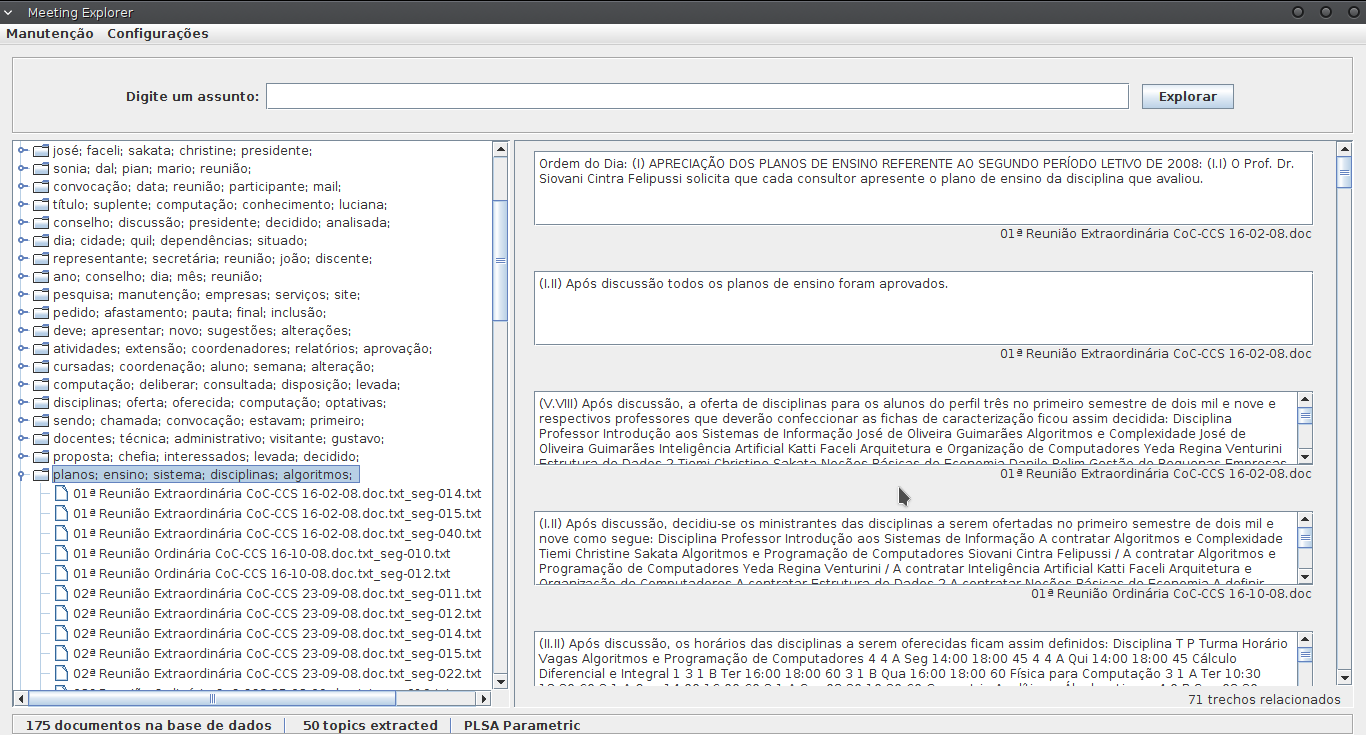
\includegraphics[width=1\textwidth]{prints/print-experimento-01.png} 
\end{figure}







% --------------------




% Trata-se de um sistema para consultas em atas de reunião. O objetivo é ajudar o usuário a fazer buscas por um assunto específico em uma coleção de atas de reunião. O Sistema deve receber uma consulta do usuário sobre um assunto e apresentar os trechos onde esse assunto é mencionado. 

% Escolheu-se as atas por tratar-se de documentos que não possuem um assunto principal, mas contém diversos assuntos registrados em um mesmo documento. Essa multiplicidade de assuntos das atas constitui um desafio para sistemas de consulta e ao mesmo tempo motivou esse trabalho de mestrado.

% Para isso, visto a multiplicidade de assuntos uma mesma ata, o sistema inicialmente  analisa a coleção de atas e divide o texto de cada ata em trechos que contêm um assunto principal e relativamente independente. 
% Ou seja, os diversos assuntos tratados em uma ata são separados em trechos com um único assunto.
% Em seguida, utiliza-se técnicas de inteligência artificial para identificar trechos com assuntos relacionados e agrupá-los. Cada grupo contém trechos de atas diferentes mas com assuntos relacionados. Além disso, o sistema seleciona um conjunto de palavras descritoras que indicam o tópico do grupo. Nesse sistema, um grupo é formado por um conjunto de trechos e por um conjunto de palavras que o descreve.

% Assim, espera-se que o agrupamento de trechos com assuntos similares extraídos de diferentes documentos facilite a navegação e busca por assuntos na coleção de atas.

% Ao iniciar, o sistema apresenta os grupos anteriormente identificados os quais são representados por suas palavras descritoras. Ao selecionar um grupo, seus trechos são exibidos ao usuário para que possa verificar o que foi registrado sobre o assunto de cada grupo. 
% %
% O sistema também permite que o usuário faça consultas à coleção de atas por meio de um campo de pesquisa por palavras-chave. Nesse caso, o sistema  analisa as similaridades entre a consulta do usuário e os trechos extraídos das atas, bem como os grupos aos quais pertence. Então, apresenta os trechos ordenados pela relevância com a consulta do usuário. Para cada trecho é apresentado além do texto, um link para o arquivo original do qual foi extraído. Ao clicar sobre o texto de um trecho, seu grupo é destacado para que o usuário possa explorar outros trechos similares.


% Abaixo é mostrado a tela principal do sistema. A esquerda são apresentados os grupos com seus descritores e a direita os trechos atribuídos ao grupo selecionado. Acima está o campo para pesquisa.

















% --> por que trechos? 

%Um trecho é representado por  texto  

%Com isso, espera-se que o agrupamento trechos de diferentes documentos, mas com assuntos similares, facilite a navegação e busca por assuntos na coleção de atas.


%Após realizar a busca, o sistema apresenta os trechos agrupados por tópicos, em que documentos com assuntos similares pertencem ao mesmo grupo. Ao selecionar um grupo, os trechos de atas são exibidos ao usuário.

%O sistema atribui um conjunto de palavras para cada grupo as quais servem para descrever o tópico do grupo.

%Cada grupo possui um conjunto de palavras 

%O sistema deve apresentar ao usuário os trechos de atas que melhor satisfazem a busca. 
 


%e documentos com assuntos diferentes ficam em gru
